\section*{BACKGROUND}
In order to experiment with robotic systems, a researcher requires a controlable robotic platform, a control system that interfaces to the robotic system and provides behaviors for the robot to carry out, and an environment to operate in.  This paper examines an opensource (the game engine is free, but license restrictions do apply), freely available framework capible of fulfilling all of these requirements. This framework is composed of the USARSim framwork that provides the robotic platform and environment, and the ROS framework that provides the control system.

\subsection*{The USARSim Framework}
USARSim~\cite{CARPIN.LNAI.2006,WANG.WSC.2003} is a high-fidelity physics-based simulation system based on the Unreal Developers Kit (UDK)~\cite{UDKWeb} from Epic Games. USARSim was originally developed under a National Science Foundation grant to study Robot, Agent, Person Teams in Urban Search and Rescue~\cite{LEWIS.ICHC.2003}. Since that time, it has been turned into a NIST led community supported open source project that provides validated models of robots, sensors, and environments.  

%Altogether, the Karma Physics engine~\cite{KarmEngine} and high-quality 3D rendering facilities of the Unreal game engine allow the creation of realistic simulation environments that provide the embodiment of a robotic system. Furthermore, USARSim comes with tools to develop objects and environments (Unreal Editor) and it is possible to control actors in the game through a TCP/IP socket API.

Through its usage of UDK, USARSim utilizes the physX phsyics engine~\cite{physXWeb} and high-quality 3D rendering facilities to create a realistic simulation environment that provides the embodiment of, and environment for a robotic
system. The current release of USARSim consists of various environmental models, models of commercial and experimental robots, and sensor models. High fidelity at low cost is made possible by building the simulation on top of a game engine. By loading the most
difficult aspects of simulation to a high volume commercial platform (available for free to most users) which provides superior visual rendering and physical modeling, full user effort can be devoted to the robotics-specific tasks of modeling platforms, control systems, sensors, interface tools and environments. These tasks are in turn accelerated by the advanced editing and development tools integrated with the game engine. This leads to a virtuous spiral in which a wide range of platforms can be modeled with greater fidelity in a short period of time.

USARSim was originally based upon simulated environments in the Urban Search And Rescue (USAR) domain. Realistic disaster scenarios as well as robot test methods were created (Figure~\ref{TestRoom}).
Since then, USARSim has been used worldwide and more environments have been developed for different purposes. Other environments such as the NIST campus (Figure~\ref{3D_World-b}) and factories (Figure~\ref{3D_World-c}) have been used to test the performance of algorithms in different efforts~\cite{WANG.HFES.2005,BALAGUER.IROS.2008,KOOTBALLY.ITEA.2010}. The simulation is also widely used for the RoboCup Virtual Robot Rescue Competition \cite{RoboCupWeb} and the IEEE Virtual Manufacturing and Automation Challenge \cite{VMACWeb} and has been applied to the DARPA Urban Challenge (Figure~\ref{3D_World-a}).

\begin{figure}[t!]
\centering
\subfigure[Test Room,]{\label{TestRoom}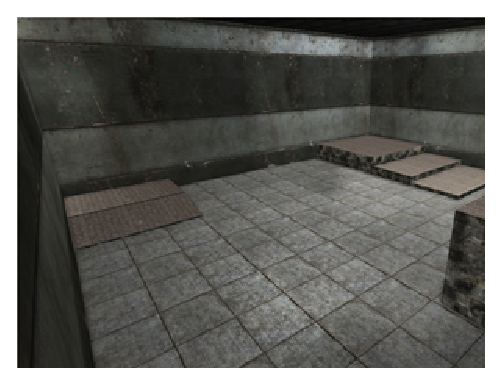
\includegraphics[width=4cm]{Figures/Worlds/testRoom.eps}}\qquad
\subfigure[NIST main
campus.]{\label{3D_World-b}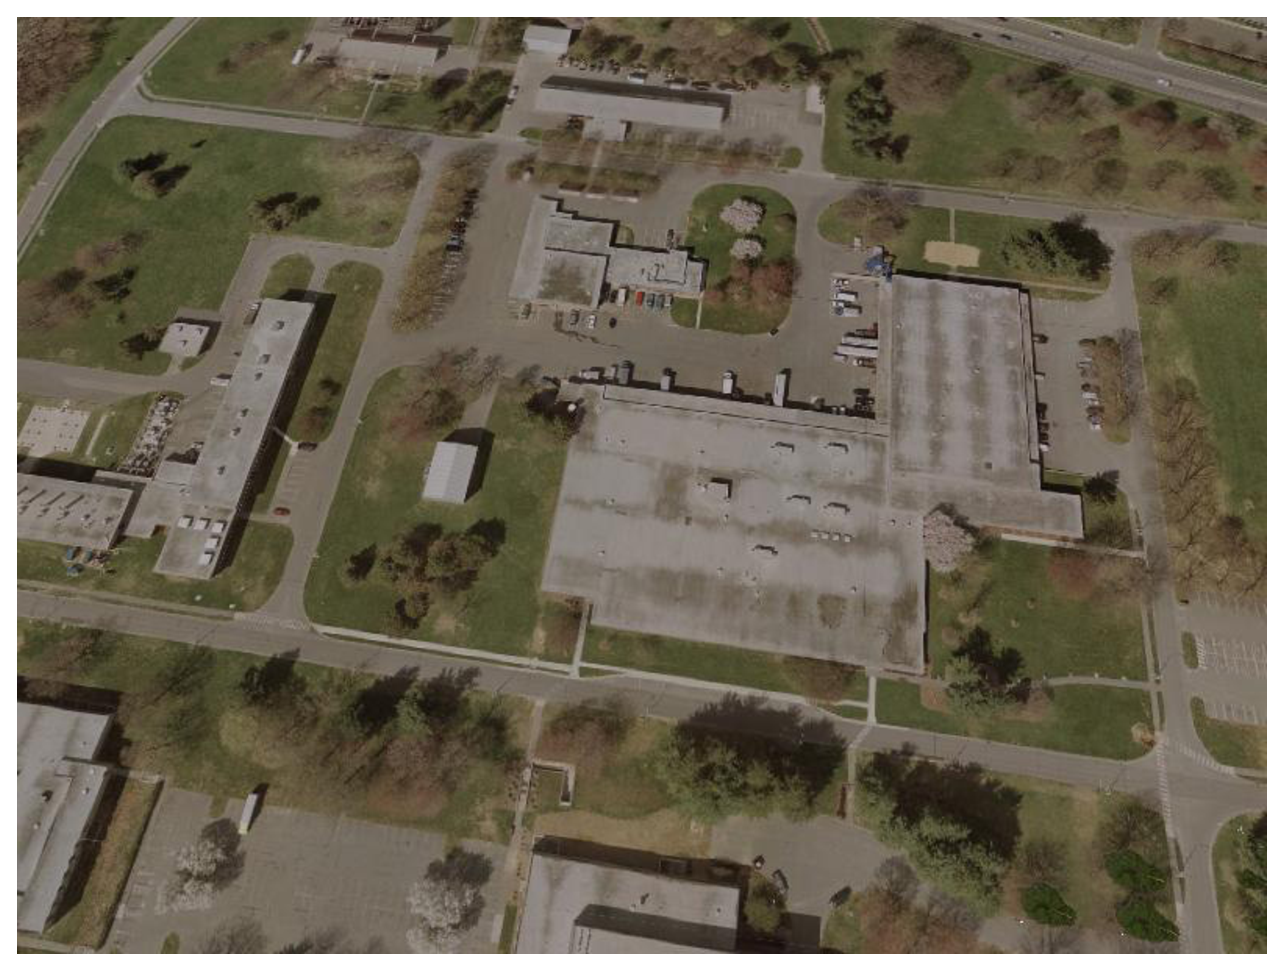
\psfig{file=Figures/Worlds/nist1.eps,width=4cm}}\qquad
\subfigure[Factory,]{\label{3D_World-c}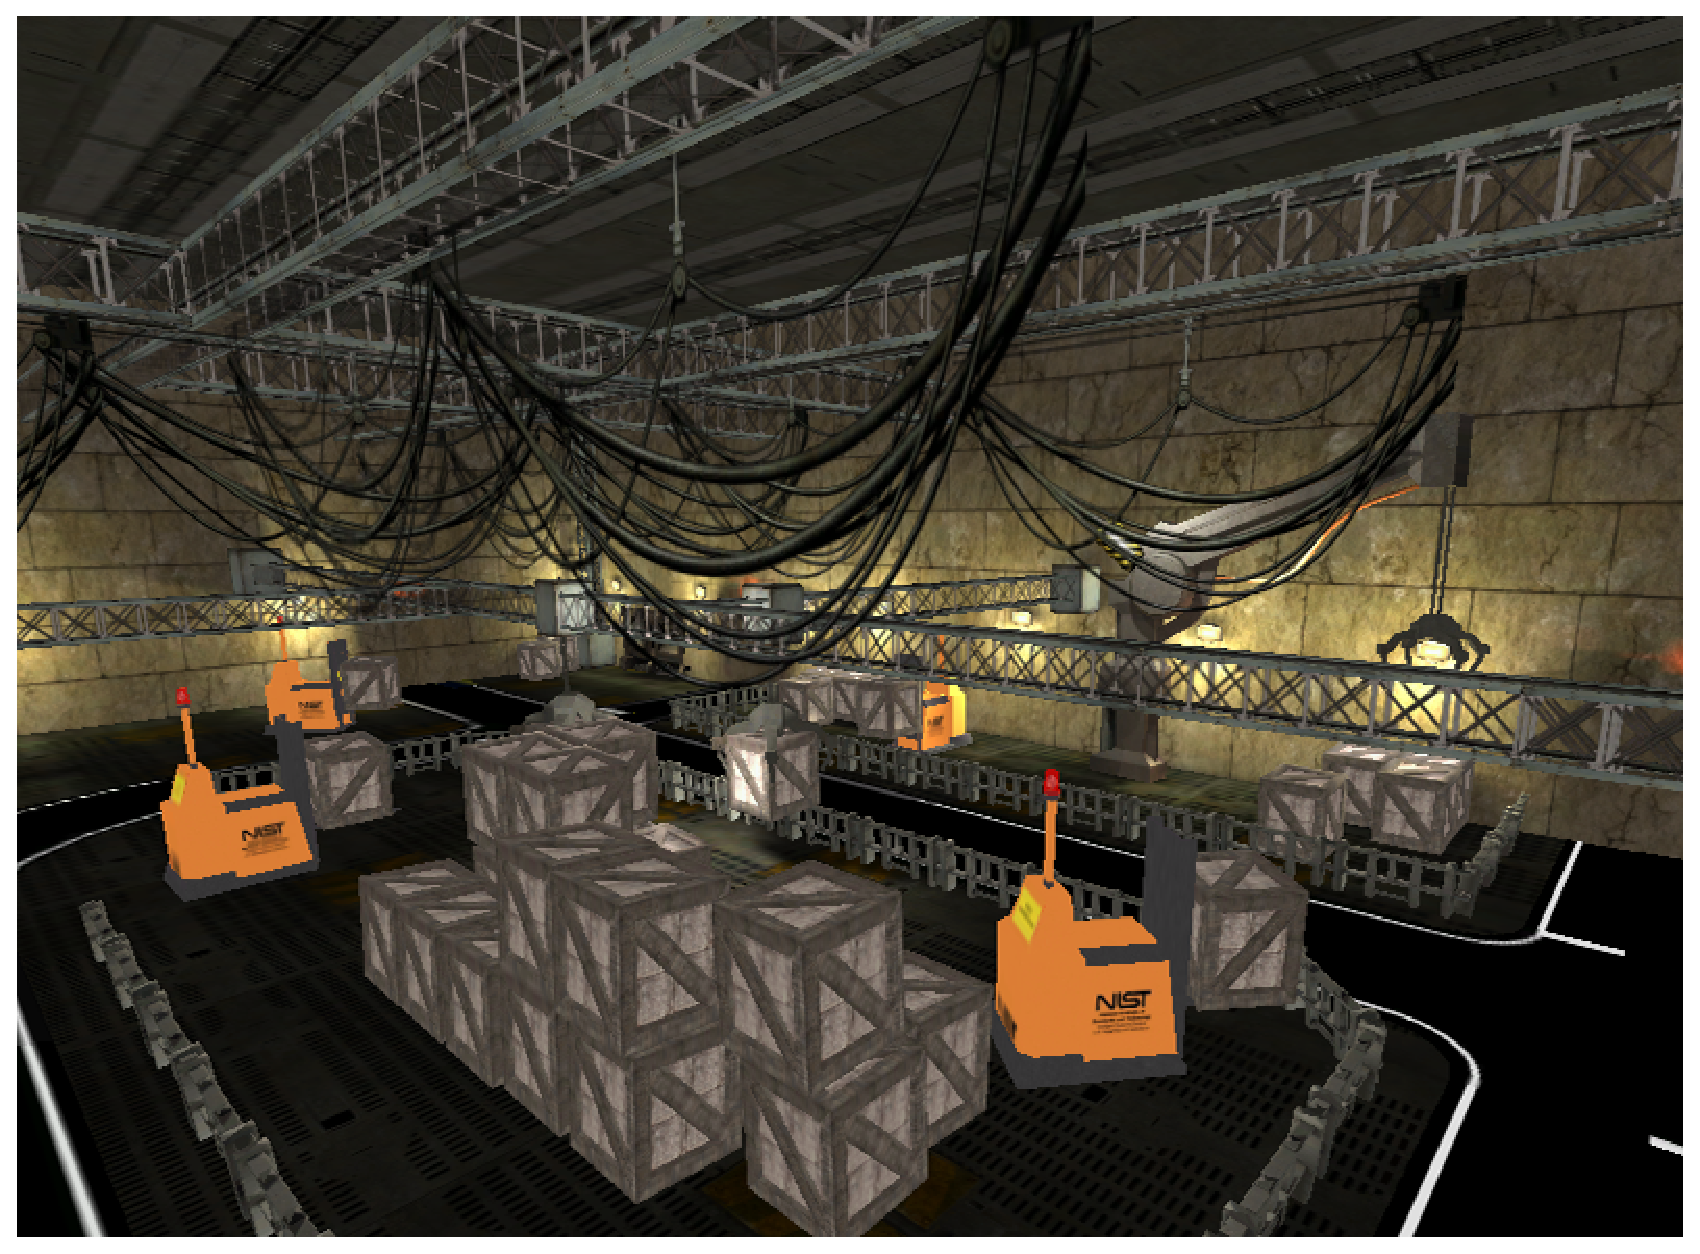
\psfig{file=Figures/Worlds/factory.eps,width=4cm}}\qquad%
\subfigure[ARDA.]{\label{3D_World-a}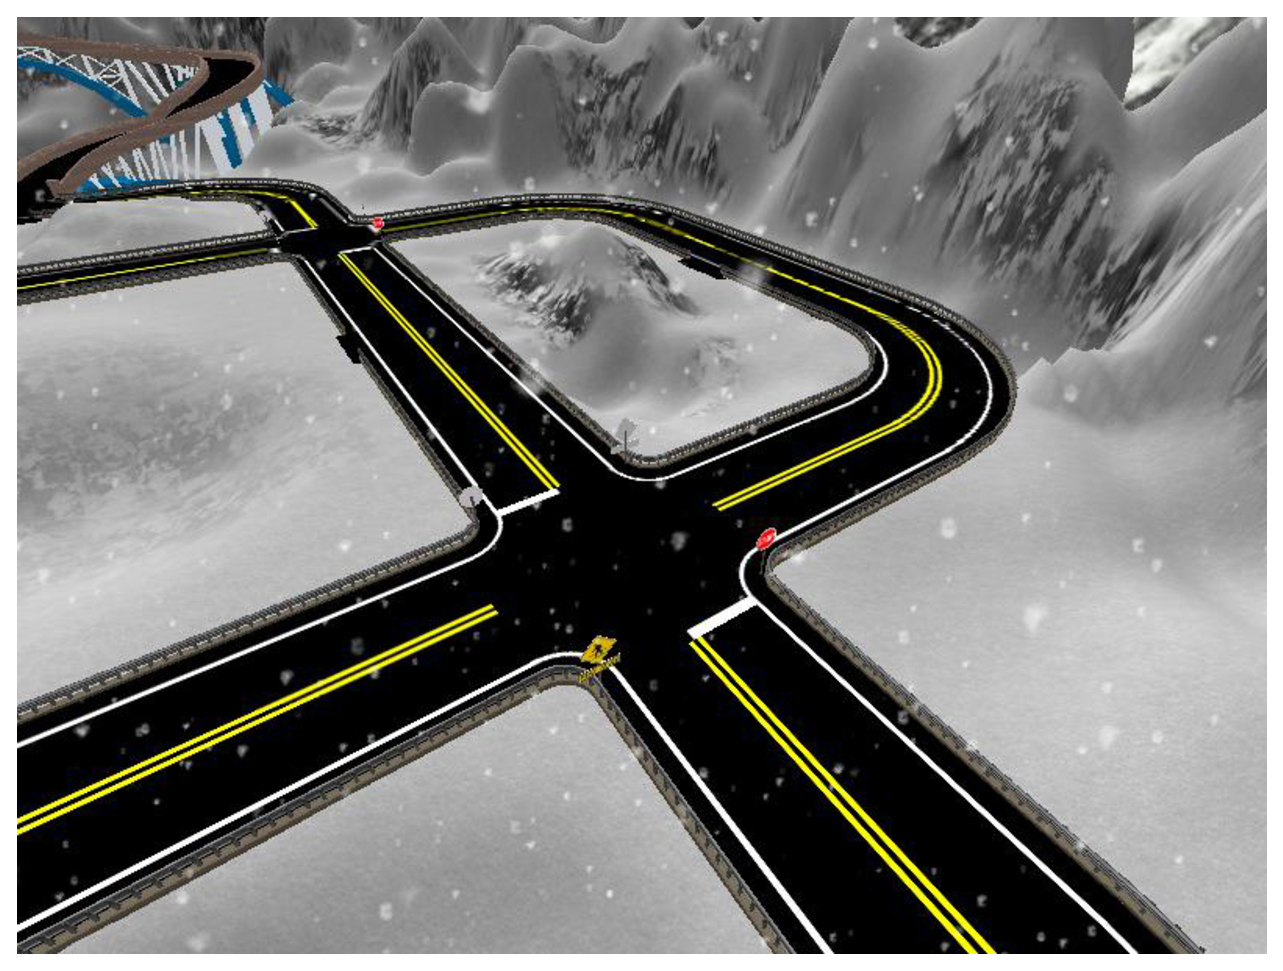
\psfig{file=Figures/Worlds/arda1.eps,width=4cm}}
\caption{Sample of 3D environments in USARSim.} \label{3D_World}
\end{figure}

USARSim was initially developed with a focus on differential drive wheeled robots. However, USARSim's open source framework has encouraged wide community interest and support that now allows USARSim to offer multiple robots, including humanoid robots (Figure~\ref{Fig:Nao}), aireal platforms (Figure~\ref{Fig:AirRobot}), robotic arms (Figure~\ref{Fig:KR60}), and commercial vehicles (Figure~\ref{Fig:Kiva}). In USARSim, robots are based on physical computer aided design (CAD) models of the real
robots and are implemented by specialization of specific existing classes. This sturcture allows for easier development of new platforms that model custom designs.

All robots in USARSim have a chassis, and may contain multiple wheels, sensors and
actuators. The robots are configurable (specify types of
sensors/end effectors for example) through a configuration file that is read at runtime. The properties of the robots can
also be configured, such as the battery life and the frequency of
data transmission.

\begin{figure}[t!]
\centering
\subfigure[ Aldebaran Robotics Nao.]{\label{Fig:Nao}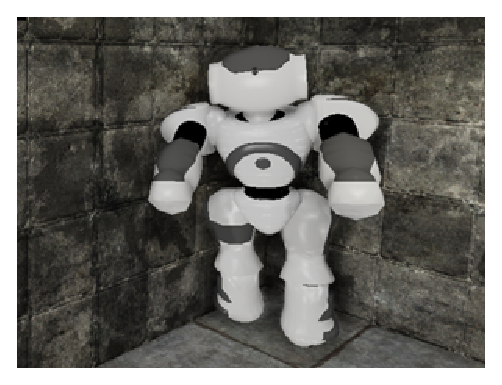
\includegraphics[width=4cm]{Figures/Robots/nao.eps}}\qquad
\subfigure[Air Robot AR100B.]{\label{Fig:AirRobot}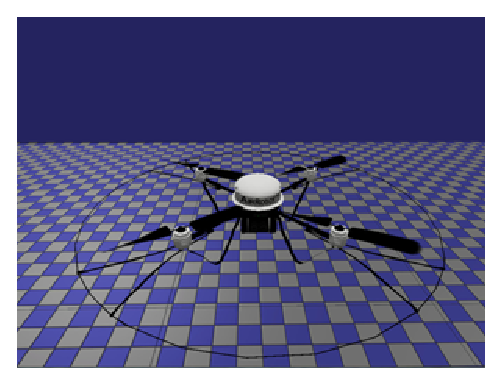
\includegraphics[width=4cm]{Figures/Robots/airRobot.eps}}\qquad
\subfigure[ Kuka KR60,]{\label{Fig:KR60}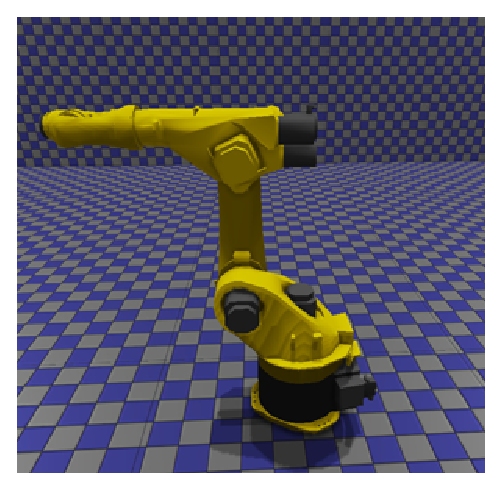
\includegraphics[width=4cm]{Figures/Robots/kr60.eps}}\qquad
\subfigure[Kiva Robot.]{\label{Fig:Kiva}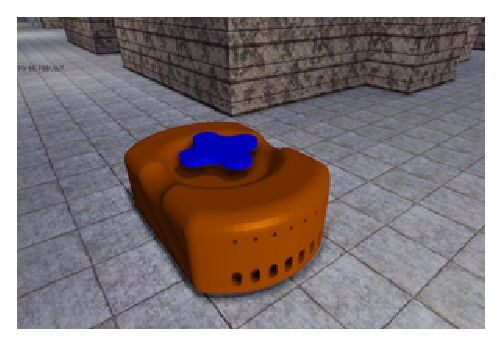
\includegraphics[width=4cm]{Figures/Robots/kiva.eps}}
\caption{Sample of vehicles in USARSim.}
\end{figure}

\subsection*{The ROS Framework}

ROS~\cite{ROSWeb} is an open source framework designed to provide an abstraction layer to complex robotic hardware and software configurations. ROS delivers libraries and tools to help software developers create robot applications. ROS has been used in many robotic applications such as
Willow Garage's Personal Robots Program~\cite{WYOBEK.ICRA.2008} and the Stanford University STAIR project~\cite{QUIGLEY.AAAI.2007}.

ROS possesses a large range of tools and services that both users and developers alike can benefit from. The philosophical goals of ROS include an advanced set of criteria and can be summarized as: peer-to-peer, tools-based, multi-lingual, thin, and free and open-source~\cite{QUIGLEY.ICRA.2009}. Furthermore, debugging at all levels of the software is made possible with the full source code of ROS being publicly available. Thus, the main developers of a project could benefit from the community and vice-versa.

\subsubsection*{Nomenclature}

ROS uses the concept of stacks, packages, nodes, messages, topics, and services. These terms are used throughout the rest of the paper and are detailed below~\cite{QUIGLEY.ICRA.2009}.
\begin{itemize}
\item[-] Node: An executable unit which communicates with other nodes. In this context, the
term ``node" is interchangeable with ``software module". Nodes communicate with each other by passing messages.
\item[-] Message: A strictly typed data structure. Standard
primitive types (integer, floating point, boolean, \ldots) are
supported, as are arrays of primitive types and constants. A node sends a message by publishing it to a given topic.
\item[-] Topic: A communication channel between two or more
nodes. A node that is interested in a certain kind of data will subscribe
to the appropriate topic. There may be multiple concurrent
publishers and subscribers for a single topic, and a single
node may publish and/or subscribe to multiple topics.
\item[-] Service: A remote procedure call defined by a string name and a pair
of strictly typed messages: one for the request and one for
the response.
\item[-] Package: A compilation of nodes that can easily be compiled and ported to other computers. Packages are necessary to build a complete ROS-based robot control system.
\item[-] Stack: Packages in ROS are organized into ROS stacks. Whereas the goal of packages is to create minimal collections of code for easy reuse, the goal of stacks is to simplify the process of code sharing. Stacks are the primary mechanism in ROS for distributing software. Each stack has an associated version and can declare dependencies on other stacks. These dependencies also declare a version number, which provides greater stability in development.

\end{itemize} 